\documentclass{standalone}
% translate with >> pdflatex -shell-escape <file>

% This file is an extract of the PGFPLOTS manual, copyright by Christian Feuersaenger.
% 
% Feel free to use it as long as you cite the pgfplots manual properly.
%
% See
%   http://pgfplots.sourceforge.net/pgfplots.pdf
% for the complete manual.
%
% Any required input files (for <plot table> or <plot file> or the table package) can be downloaded
% at
% http://www.ctan.org/tex-archive/graphics/pgf/contrib/pgfplots/doc/latex/
% and
% http://www.ctan.org/tex-archive/graphics/pgf/contrib/pgfplots/doc/latex/plotdata/

\usepackage{pgfplots}
\usepackage{pgfplotstable}
\pgfplotsset{compat=newest}

% The manual loads these libraries globally; the extracted standalone examples
% need them too. external/clickable/snakes are intentionally omitted.
\usetikzlibrary{
	arrows.meta,backgrounds,calc,decorations.footprints,decorations.markings,
	decorations.pathreplacing,fixedpointarithmetic,intersections,patterns,
	plotmarks,shapes.arrows,spy,through}
\usepgfplotslibrary{
	colorbrewer,colormaps,dateplot,fillbetween,groupplots,patchplots,polar,
	smithchart,statistics,ternary,units}

% Some colormap examples reuse this display style defined earlier in the manual.
\pgfplotsset{
	cycle from colormap manual style/.style={
		x=3cm,y=10pt,ytick=\empty,
		colorbar style={x=,y=,ytick=\empty},
		point meta min=0,point meta max=1,
		stack plots=y,
		y dir=reverse,colorbar style={y dir=reverse},
		every axis plot/.style={line width=2pt},
		legend entries={0,...,20},
		legend pos=outer north east,
	},
}

\pagestyle{empty}
\usepackage{pgfplotstable}

\begin{document}
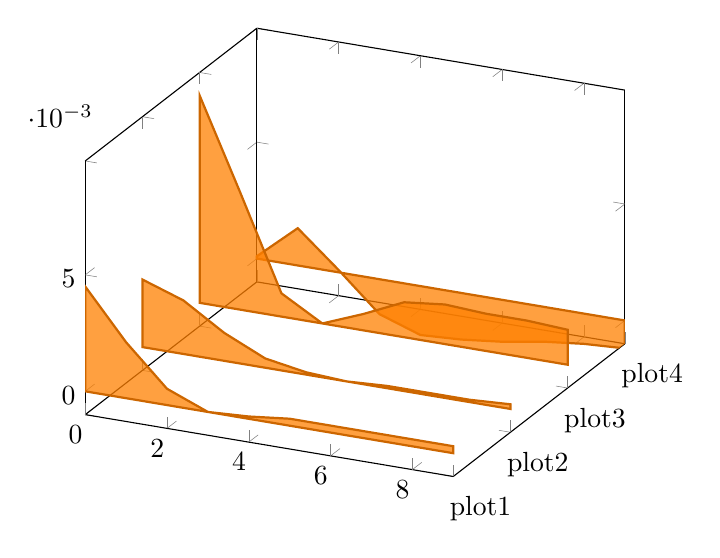
\begin{tikzpicture}
\pgfplotstableread{
plot1     plot2     plot3     plot4
0.0045    0.0029    0.0089    0.0001
0.0024    0.0023    0.0050    0.0016
0.0007    0.0012    0.0010    0.0001
0.0000    0.0004   -0.0000   -0.0015
0.0001    0.0001    0.0007   -0.0021
0.0003    0.0000    0.0015   -0.0020
0.0003    0.0001    0.0017   -0.0018
0.0003    0.0001    0.0016   -0.0015
0.0003    0.0001    0.0016   -0.0013
0.0003    0.0002    0.0015   -0.0012
}\tabledata
\begin{axis}[
    zmin=-0.001,
    area plot/.style={
        fill opacity=0.75,
        draw=orange!80!black,thick,
        fill=orange,
        mark=none,
    },
    ytick={1,...,4},
    yticklabel=plot\pgfmathprintnumber{\tick},
]
    \pgfplotsinvokeforeach{4,3,...,1}{
        \addplot3 [area plot] table [
            x expr=\coordindex, y expr=#1, z=plot#1,
        ] {\tabledata} \closedcycle;
    }
\end{axis}
\end{tikzpicture}
\end{document}
